\begin{enumerate}[label=\arabic*.,ref=\theenumi]
	\item The following instructions are for the picow toolchain
		in debian
\begin{lstlisting}
cd .platformio/packages
git clone https://github.com/earlephilhower/arduino-pico
cd arduino-pico
git submodule update --init
cd pico-sdk
git submodule update --init
cd ../tools
python3 ./get.py
\end{lstlisting}
\item Now execute the following 
\begin{lstlisting}
cd picow/installation/codes/src/main.cpp
pio run
\end{lstlisting}
% Insert your image here
		\begin{figure}
			\centering
    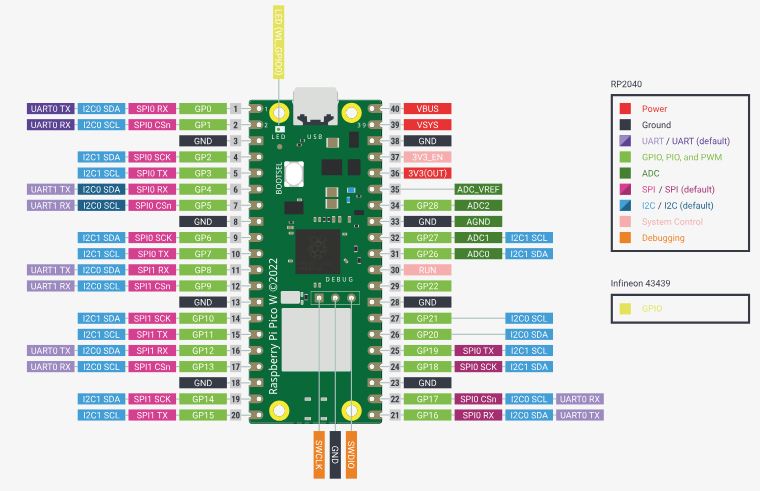
\includegraphics[width=\columnwidth]{picow/installation/figs/picowpinout.jpg}
    \caption{Pico Pin Diagram} % Adds a centered caption under the image
			\label{fig:picowpinout}
		\end{figure}
\item Connect RUN on pico W to GND. Keep pressing BOOTSEL while removing the RUN-GND wire from GND.Pico W is now ready to be flashed.
\begin{lstlisting}
Downlaod EtchDroid from playstore.Flash the uf2 file using EtchDroid.
\end{lstlisting}
\item The Onboard LED will start blinking.
\end{enumerate}





